In order to show an improvement on existing predictive simulation systems for CHD corrective surgeries, we want to demonstrate that our blood vessel model based on thin shell elements
\begin{enumerate}
\item physically meets the requirements for predictive simulation results,
\item converges to these results with a low number of elements,
\item is able to universally simulate low-level surgical procedures.
\end{enumerate}
We close this section with a discussion about limitations and constraints of our simulation approach in terms of generation and dynamic remeshing of thin shell element meshes.

A quantitative validation by means of a comparison to real pre- and post-surgery image data is impossible at present. This is mainly due to ethical issues that arise during image data acquirement of infants, i.e. necessary heart rate lowering medications or exposure to radiation. There is no such data available that is obtained shortly after surgeries in infants where the growth of the patient would not interfere comparison. However, a qualitative comparison to real image data acquired months after a surgical intervention, which confirms a principal suitability of predictive simulations for surgery planning, can be found in \cite{Li2009}.

\subsection{Predictive Simulation Results}

\begin{figure}[tbh]
    \centering
    \begin{tabular}{cc}
     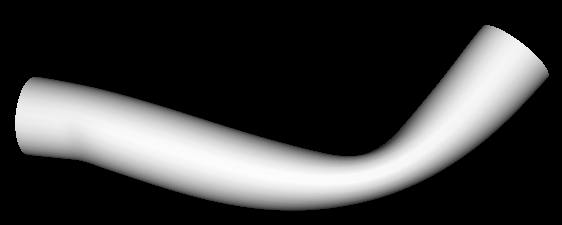
\includegraphics[width=0.4\columnwidth]{img/compare-bend.png}
      &
      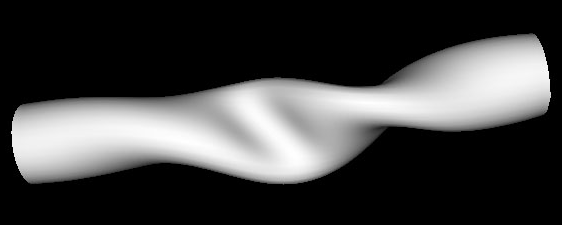
\includegraphics[width=0.4\columnwidth]{img/compare-twist.png}
      \\
      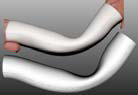
\includegraphics[width=0.4\columnwidth]{img/compare-bend-other.png}
      &
      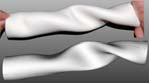
\includegraphics[width=0.4\columnwidth]{img/compare-twist-other.png}
    \end{tabular}
    \caption{Simulation of bending and twisting of an elastic tube. Top row: Thin shell element model; Bottom row: Real elastic tube manipulated by hand and Cosserat rod-based hybrid model \cite{Li2009} (Credits for the bottom images: Li et al.).}
    \label{fig-deformations}
\end{figure}

Figure \ref{fig-deformations} shows bending and twisting of an elastic tube manipulated by hand compared to the simulation results of \cite{Li2009} and our method. These kinds of blood vessel deformations are likely to occur during surgery. Our results are close to the real deformations as expected due to the physically based formulation of thin shell elements.

\subsection{Convergence}

\begin{figure}[tbh]
  \centering
  \begin{tabular}{cccc}
    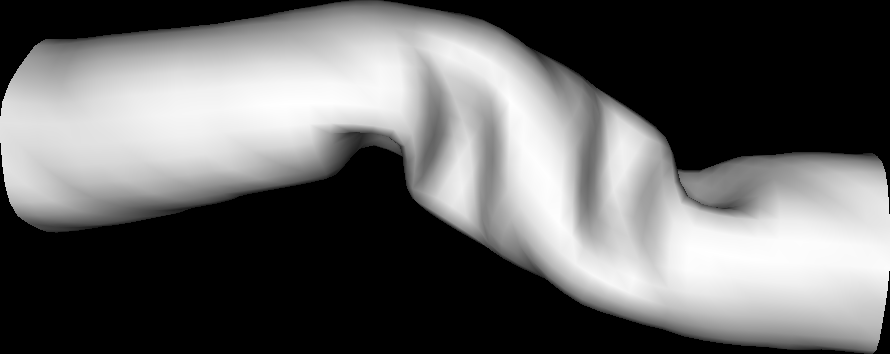
\includegraphics[width=0.48\columnwidth]{img/twist-06-cg.png}
    &
    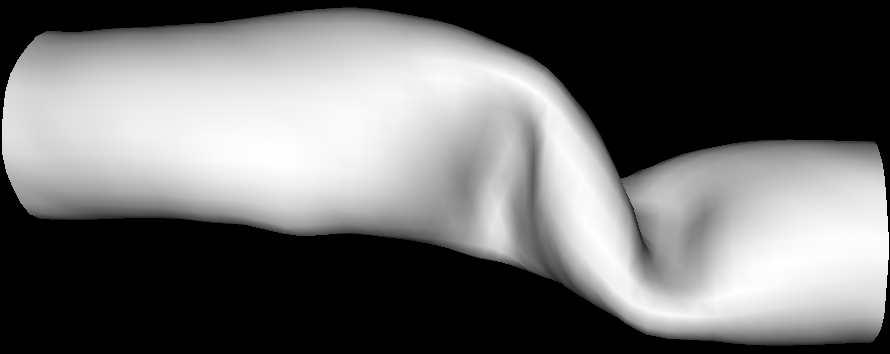
\includegraphics[width=0.48\columnwidth]{img/twist-08-cg.png} 
    \\
    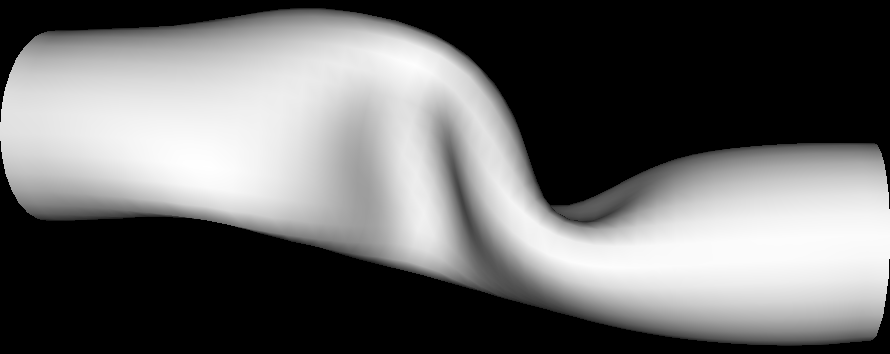
\includegraphics[width=0.48\columnwidth]{img/twist-16-cg.png}
    &
    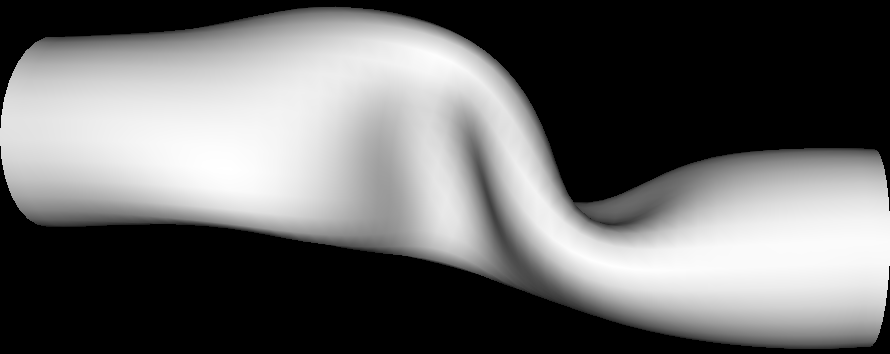
\includegraphics[width=0.48\columnwidth]{img/twist-31-cg.png}
    \\
    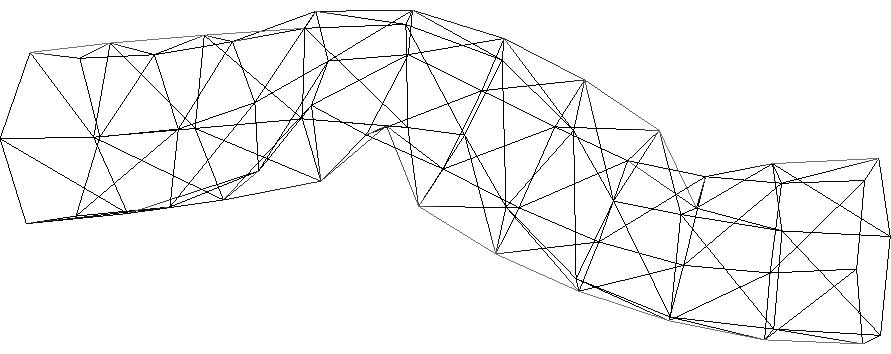
\includegraphics[width=0.48\columnwidth]{img/twist-06w-cg.png}
    &
    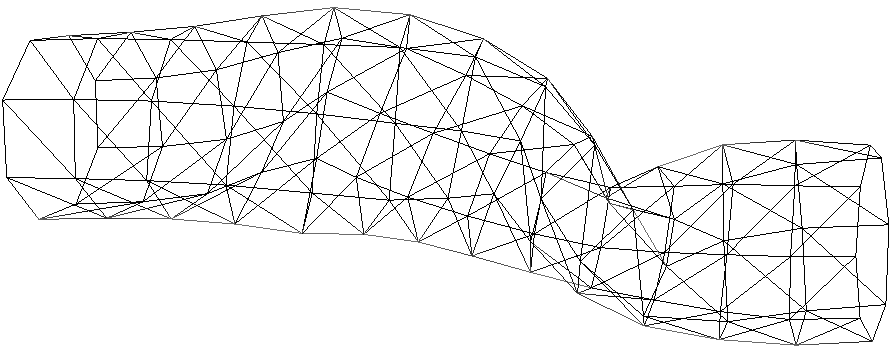
\includegraphics[width=0.48\columnwidth]{img/twist-08w-cg.png}
    \\
    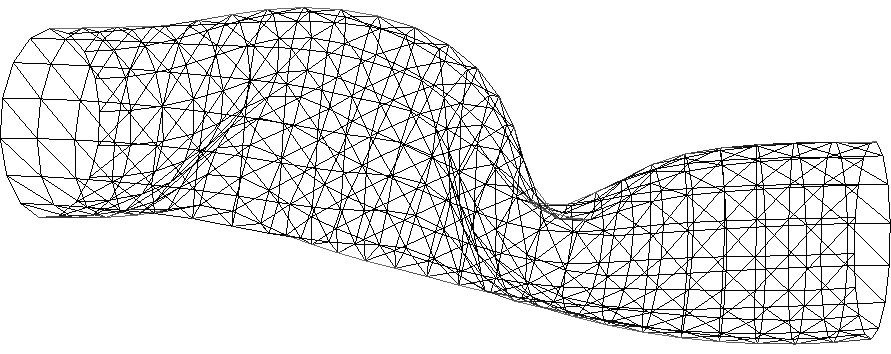
\includegraphics[width=0.48\columnwidth]{img/twist-16w-cg.png}
    &
    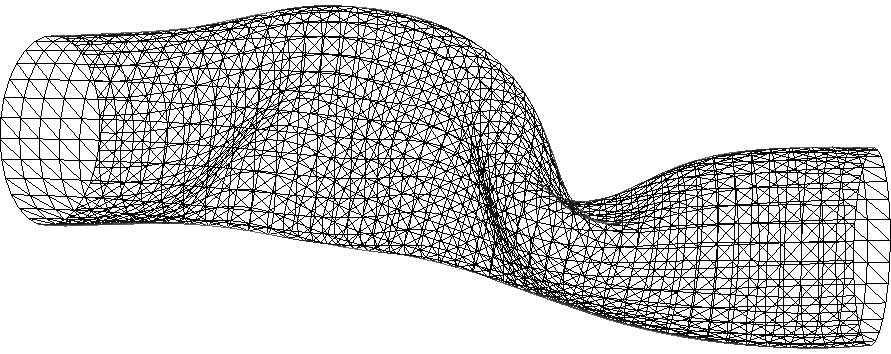
\includegraphics[width=0.48\columnwidth]{img/twist-31w-cg.png}
  \end{tabular}
  \caption{Convergence of a twisted, elastic tube with 6, 8, 16 and 31 vertices
  along its circumference (120, 208, 832 and 3038 thin shell elements). Top row: High polygon count mesh mapped to simulation results of coarser shell element meshes (bottom row).}
  \label{fig-convergence}
\end{figure}

It is important to minimize the number of shell elements to reduce computation time. This is the key factor to enable an interactive simulation system that is accepted by surgeons to simulate multiple surgical approaches in succession. The bending capabilities of thin shell elements allow to reduce their number and still representing the tubular structure of blood vessels while maintaining their physical behavior appropriately. Figure \ref{fig-convergence} shows simulation results of a strongly deformed tube represented by different numbers of thin shell elements. With only eight vertices along the circumference of the elastic tube the simulation result is comparable to a simulation result with high element count.

\subsection{Low-Level Surgical Procedures}

\begin{figure}[tbh]
  \centering
  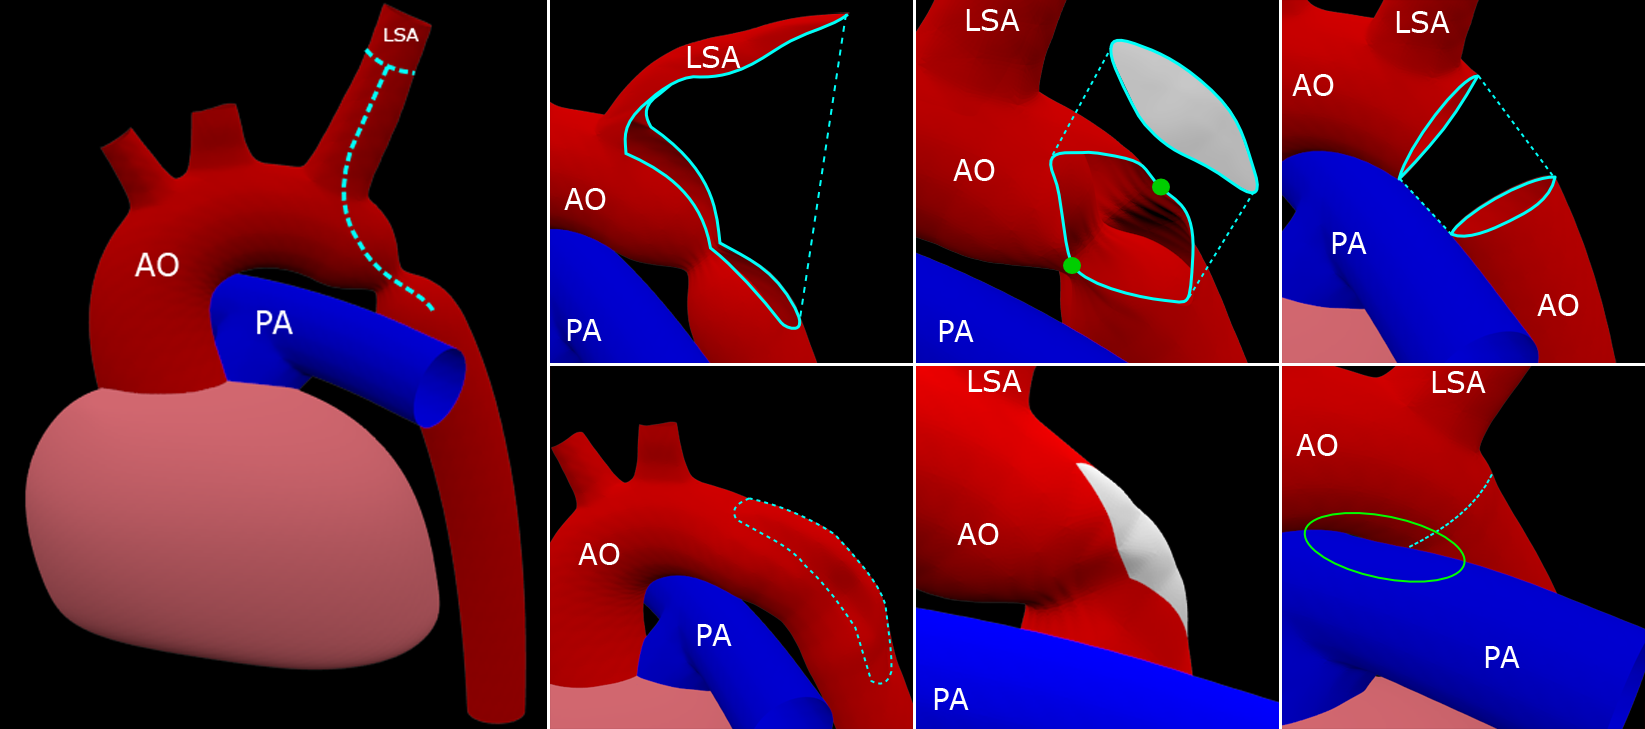
\includegraphics[width=\columnwidth]{img/surgery.png}
  \caption{Simulation of different surgical procedures for coarctation repair of an aortic arch. Left image: Overview of the simulation scene consisting of an aortic arch (AO), a left subclavian artery (LSA) and a pulmonary artery (PA). The coarctation can be seen next to the LSA and the dashed line indicates where the aorta is to be incised for a subclavian flap aortoplasty; The vertical image pairs show the scene before and after different surgical interventions. From left to right: Subclavian flap aortoplasty -- the subclavian flap is used as an organic onlay patch over the area of coarctation; Patch aortoplasty -- the incision is opened by attached springs only for visualisation purposes. The patch is sutured in place as shown; End-to-end anastomosis -- the coarctation is resected and the loose ends of the AO sutured together. Due to deformation of the AO there is a collision with the PA, causing slight deformations on both blood vessels. }
  \label{fig-surgery}
\end{figure}

We manually modeled an aortic arch based on real image data to be able to demonstrate suitability of our joining approach for different kinds of low-level surgical procedures on a concrete example. Therefore we chose a coarctation of an aortic arch that can be repaired by several different surgical approaches that heavily alter the surface of the blood vessel \cite{Dodge2000}. Results can be examined in figure \ref{fig-surgery}. We show that our topological method for joining of shell elements through a controlled relaxation to their rest shape is able to handle different kinds of connections universally and in a correct manner.

\subsection{Limitations and Constraints}

Finite element methods including thin shell elements have some constraints in common regarding the simulation mesh quality. A homogeneous neighborhood of equally sized elements is desirable. Especially when minimizing the number of elements, high mesh quality is necessary to maintain convergence and stability of the simulation. We showed that an elastic tubular structure can be simulated appropriately for CHD corrective surgeries with only a few elements. To allow for arbitrary incisions under such circumstances, the mesh must be remeshed in a way that its elements align along an incision. Mesh quality must be retained during remeshing and therefore the whole mesh may be affected. A limitation of our joining approach is that we need the same number of elements along connecting edges. Appropriate remeshing strategies must be developed to take full benefit of our proposed simulation approach. However, as a fall-back, element count could be increased which will have negative impact on the simulation speed.

%Example with 3 diff. surgical procedures
%Parameters
%Limitations (getting image data, meshes, dynamic remeshing, same number of nodes)
